\chapter{Implementation}
This chapter describes the implementation of a prototype of the system.
It shows how each component was implemented to deal with the requests' limits of external services.
Then, the interaction between them is explained showing the data flow starting with the user request to the final response.
Finally, the techniques used for each classifier are introduced.

\section{Components interactions}
Generally, the system is composed by a main request which mobilizes the download of a user's profiles, their analysis and finally their classification.
This process ends with a series of classified batches, of monthly time duration, that are stored in the database.
Then, the call to obtain the final results starts the insight generator shown in Section~\ref{sec:Generator} which merges together the partial results and return the final insight at the user level.

These different types of requests are handled by the request handler which is represented by the user's endpoint, the only interface to the outside of the system.
As said before, it also allows to add and modify the system's users.
The download request is the one that requires communication between multiple components.

This prototype allows the interaction and the download of social profiles only from Twitter.
Indeed, while data from Twitter are publicly accessible through its APIs, other social media, such as Facebook and Instagram, require an access token for each consulted user.
To obtain the access token, a demo video that shows what the system does must be provided, the data treatment has to be described precisely, and each person should accept to share its data.
\subsection{Download Request}
\label{sec:downloadRequ}
The endpoint /newactivities represents the most complex one that involved the majority of the components.
In this prototype, the components execute synchronously. In the moment the request is received, the activities collector is executed and the system waits for it to end and return its results.
Then, all the downloaded activities are analysed. Once all the features are extracted, they are divided in batches and finally classified and stored.

The process starts with the ID of a user which is used to search on the database the Twitter ID associated with that specific user. 
This is used by the activities collector to download the new content. As said before, the system is structured to download only new activities and not the whole timeline.
To do it, it is used the ID of the oldest activity of the second-to-last stored batch because the last one could contain only a part of the content posted in a month. 
The drawback of this choice is that activities already contained in the last batches are downloaded and classified again but it is necessary to ensure a full download. Moreover, a maximum of thirty days is downloaded twice which is a limited number compared to the whole user's timeline.
The collector uses \textit{Tweepy}, a Python library, to access the Twitter API. It allows to download a user's content specifying its ID and the point from where the download of its activities should start.
Once the download is complete, an object \textbf{User} is created. It contains both social information about the profile, such as creation date and description, and the list of all the fetched activities. Each one is represented by a \textbf{Post} object that contains everything about the downloaded content: creation date, number of likes and retweets, its text, list of media, hashtags and urls.
The user object is passed to the next component, the analyser, with a standard class method call by the request handler.

The analyser is the component that extracts, starting from the single activities, the significant features.
Considering the various classifiers implemented, different types of features are extracted.

First of all, the information contained into the fetched tweet object that does not require any processing or further analysis is kept also in the analysed Post. This includes its id, the creation date, the number of favourites and retweets, the language of the tweet, and its type.
There are 4 different types of tweets: original, reply, retweet, and quote.

The text component of the post is used to obtain fundamental textual features. This analysis is carried out using \textit{SpaCy}, an open-source Python library for natural language processing.
Before executing the Spacy pipeline, some pre-processing is done. Whitespaces are normalized, multiple spaces and new lines are treated as a single space. The number of capital letters is memorized and then the text is converted completely in small caps.
Then, the text is passed through all the components of the pipeline. It starts with the \textit{tokenizer} which segments text into tokens like words and punctuations marks. The \textit{lemmatizer} is now involved to reduce each word to its canonical form, called \textbf{lemma}. Then, each token is assigned a part-of-speech tag thanks to the \textit{tagger}.
At this point, 2 custom components are added. First, the extension \textit{spacymoji} is used to handle emojis efficiently. Then, the last component handles \#hashtags and @mentions so that the lemma does not contain special symbols \# and @.
The result of this pipeline is a list of tokens that represent the bag of words extracted from the text. Each token contains information such as the raw word, its lemma, and its POS tag.
Now, other more generic features are extracted. spacy allows counting automatically the number of sentences, words, and characters. Starting from this data, many averages are computed such as number of words per sentence and characters per word.
To conclude, the tokens extracted before are divided into three different sets: words, stop words, emojis, and punctuation.
This distinction is important because we that our classification models could treat each set differently.
Stop words refer to the most common words in a language. There is no single general list of stop words and any group of words can be chosen. Spacy provides its own list for each supported language.
The punctuation set includes all the standard punctuation marks but \# and @ that are often special symbols on the social networks.
Finally, the words set contains all the other words.
Each set is memorized as a dictionary {\textbf{key} : \textbf{value}} used as a counter where \textbf{key} is the text of the token and \textbf{value} is its number of occurrences in the tweet.  
Some of the pipeline operations described, such as the lemmatizer, the tagger, and the stop words list, are language-dependent. In this prototype, the Italian module of Spacy has been used so these three specific phases are optimized only for that language. Anyway, Spacy provides plenty languages models and also a multi-language one.

Another important group of features is that describing the content of a tweet. For this purpose, \textit{DandelionAPI}, a semantic analysis service was used. It works on unstructured text to extract its meaning. 
In particular, it offers two important functionalities: entity extraction and sentiment analysis.
The first one can be useful to understand a person's interest and therefore is not used in this prototype which does not implement that specific classifier.
The second one may have an important role with respect to psychological characteristics.
It allows identifying whether an opinion contained in the tweet is negative, neutral, or positive. 
DandelionAPI is accessed with restAPIs and one request is necessary for each piece of text that need to be analysed. Moreover, it supports more than 40 languages, including Italian and English, and it can also compute automatically the language detection of the text given as parameter.
The response is structured in JSON and contains: the detected language, a sentiment score and a sentiment type.
The score is a more precise indicator ranging from -1.0 (totally negative) to 1.0 (absolutely positive) while the type is a descriptive label which can be \textit{negative}, \textit{neutral}, or \textit{positive}. 

Finally, the set of features regarding the media entities is created. Twitter supports three types of media: photos, videos and animated gifs. They are generally treated as \textit{media entity}.
The TwitterAPI returns, for each entity, a exhaustive series of descriptive attributes. Of interest for this prototype are the media type and the media URL.
The first one is important to understand in which way a person ten to communicate while the second one represents an important part of the tweet's content.
They may be analysed in order to detect emotion, entities and, places in a way similar at that done for the text.
So, even though images and videos are not used in this demo, mainly because rarity of free computer vision services, the URLs are downloaded to easily allow future improvements.

Once all the features are extracted, the same \textbf{User} object taken as input is modified replacing the list of \textbf{Post} object with a list of features which represents the analysed tweets.
This new object is passed to the next component, the aggregator.

The aggregator has to goal to divide the posts in batches and then compute the aggregates for each batch.
As introduced before, in this prototype the batches are temporality-based and each one ranges over a period of one month.
Thanks to the creation date of the posts, it is easy to divide them. Then, the information related to the social profile is copied into each batch.
At first each batch represent a partial user composed by its descriptive data and its analysed timeline.
The aggregator algorithm is executed on each batch to obtain a final classifiable object.
The system includes many various features structured in many different formats. So, there is no standard way in which these are aggregated together.
For different typologies, different approaches were applied.
For example, information about the number of favourites and retweets is given from the simple average all tweets. Textual features about the different sets of tokens are merged by summing together the single count dictionary of each activity. Then, the counters are converted to frequency with respect to the totality of words. 
Two lists are used to count the percentage of each typology of tweets and the time it was posted. Concerning the first one, four elements are enough. Differently, for the second one, it depends on which information is considered necessary.
Here is used a list of length twenty-four to keep count at which specific hour of the day the activities are posted.
In the end, the list of batches is returned and given as input to the classifiers.

The classifiers are the last step of this request. Since they share a common architecture, they take as input the same object and return the output result with a common structure.
The input of each classifier is a batch, or a list of batches. The output is usually an integer that represents the class assigned by that model.
In this prototype, the classification algorithms are executed sequentially one after the other. Each result is stored in an dictionary {\textbf{key} : \textbf{value}} where \textbf{key} is a label that identifies the classifier. For example, it can be \textit{EI} to indicate the result that regards the classification of the Extrovert/Introvert aspect or \textit{Sentiment} which is the name of the classifier that performed the person's general sentiment.
The \textbf{value} is an integer indicating the specific assigned class.
An object of this type is returned for each batch and it's integrated with other descriptive information: the month covered by the batch in the format \textit{MM-YYYY}, the number of tweets contained, and the ID of the last posted one.
As introduced in Section~\ref{sec:Classifiers}, lack of data is a serious problem that limits the use of machine learning techniques. So, only for a limited number of classifiers these techniques have been used.
For the others, the implementation followed the algorithms explained in Section~\ref{sec:Classifiers}. 

\subsection{GetUser request}
\label{sec:getUserReq}
This section describes how the second important request was implemented.
When this request is called on a classified user, its partial results of every batch are merged together applying an implementation of the algorithm~\ref{algoGenerator} and then returned.
As parameters, it requires only the ID of the system user. It returns in output, structured as JSON, the user characterised by its information and its final insights.

This involves only one component, the insight generator. It has to query the database to obtain all the partial results of the searched user and then run the algorithm described in Section~\ref{sec:Generator}.
In this prototype, each batch covers a period of exactly one month. 
The values $\gamma$ and $\delta$ are computed as follows:
\begin{gather}
\label{gamma}
\gamma = \ceil{((actualYear*12 + actualMonth) - (batchYear*12 + batchMonth)/2)} \\
\delta = batchActivities
\end{gather}
So, $\delta$ consists in only the number of activities contained in a specific batch. 
$\gamma$ is an integer that takes into consideration the number of months between the actual one and the one covered by the batch. This value starts at one and increase of one every two months.

Then the algorithm is applied with these two values, that are calculated at every iteration.
Finally, the final object representing the user can be returned.


\section{User dashboard}
\label{sec:userDash}
Finally, a dashboard to see the results and evaluate the system's efficiency was realized.
It is a web client that allows searching for a user and observe how his or her insights changed over time.

The application is realized with \textit{HTML}, \textit{JS} and uses \textit{AJAX} to communicate with the system.
The dashboard send a getUser request~\ref{sec:getUserReq} and display the results in a readable way.
For each classification, a stepped line graph is used. On the x-axis, there are the months covering the whole user's timeline.
On the y-axis, there are the classes depending on which classification is being observed.

Figure~\ref{fig:userDash} shows a view of the dashboard for a random user. The displayed classification is that of the used language. It is observable that the user tend to communicate only in Italian and English.

\begin{figure}[htp]
    \centering
    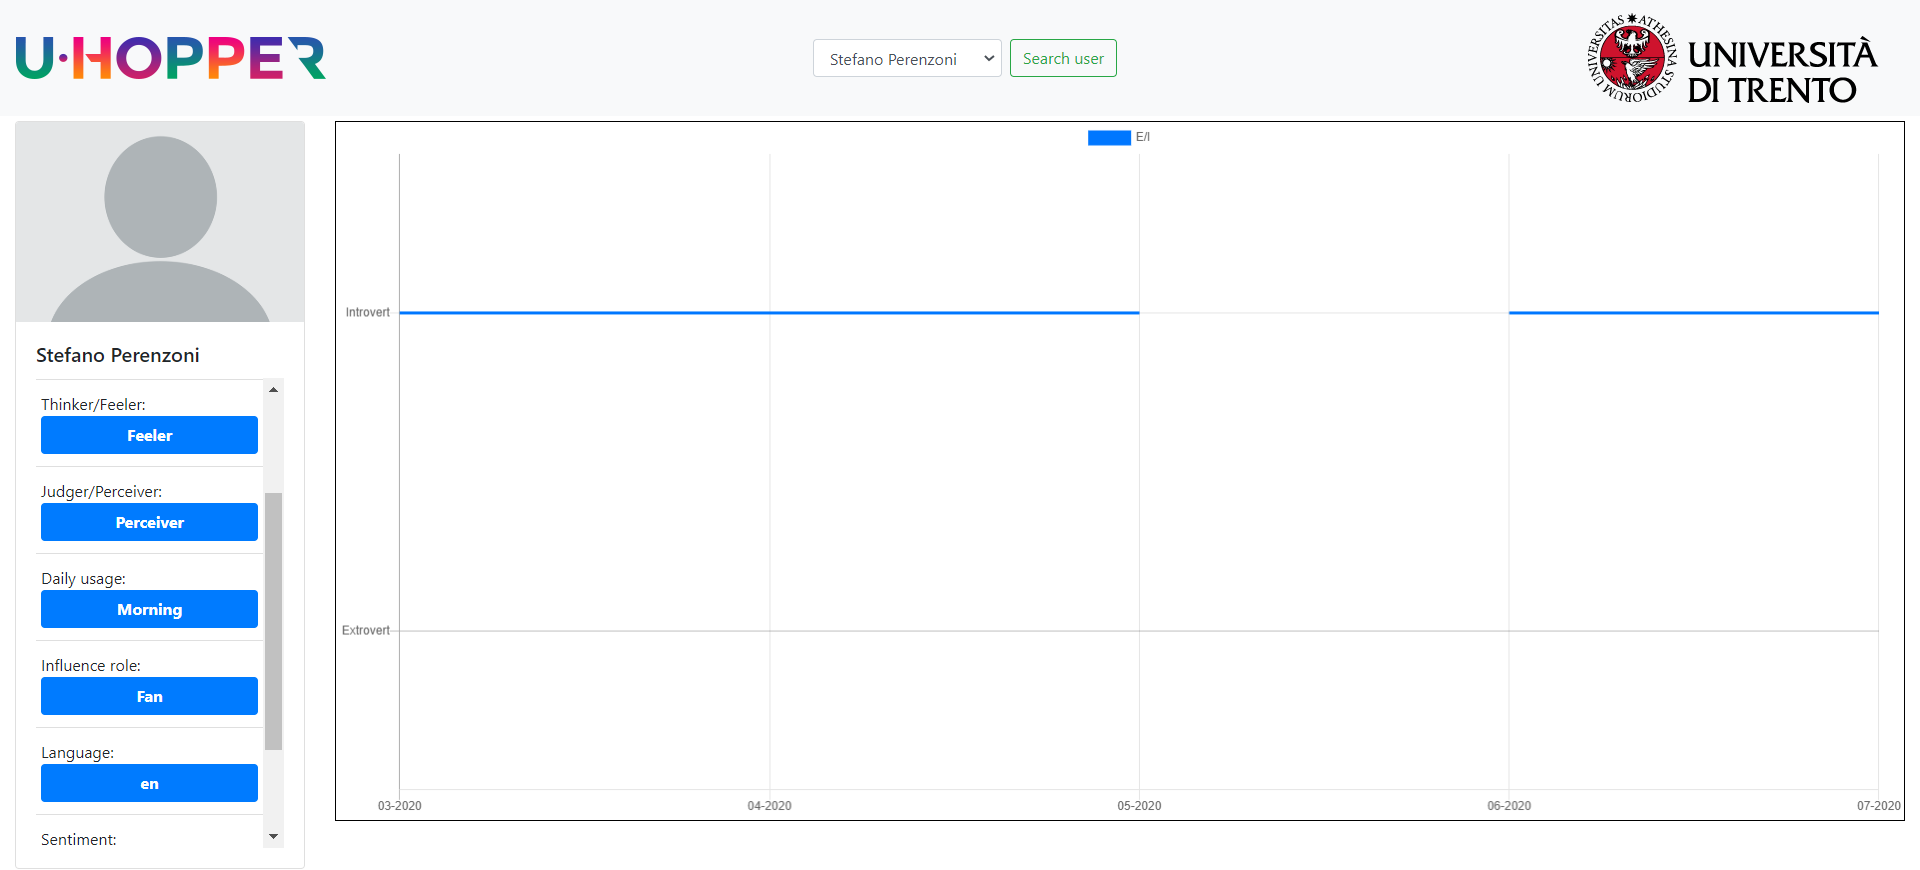
\includegraphics[width=%
    0.95\textwidth,height=20cm,keepaspectratio]{img/userDash}
    \caption{A view of the user dashboard}
    \label{fig:userDash}
\end{figure}